\documentclass{assignment-373}
\usepackage{mathabx}
\usepackage{tikz}


\anum{1}
\course{CSC373}
\duedate{Oct 7, 2022}
\filename{ps1.pdf, ps1.tex}

\begin{document}

\think

\textbf{Please see the course information sheet for the late submission
  policy.}

\begin{enumerate}
\item \textbf{[15 points]}

  Sushant finds crosswords fascinating. However, rather than attempt
  to solve the word clues, he enjoys finding patters in the crossword
  grid.
  So whenever he sees a crossword grid, he's
  looking to find the biggest diagonal he can fit in it.

  You are given an $n \times n$ array with entries in 0 or 1. 0
  indicates that that location is empty, and 1 indicates that the
  location is filled. Your goal is to determine the largest diagonal
  that can be filled in the grid while utilizing only the 0
  locations. The following figures below demonstrate diagonals with
  sizes 1, 2, 2, 3, and 3 respectively (a zero sized diagonal would have no
  blue squares). Note that the diagonal can go from top-left to
  bottom-right, or bottom-left to top-right.
  
  \begin{minipage}{1cm}
    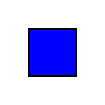
\begin{tikzpicture}
      [%%%%%%%%%%%%%%%%%%%%%%%%%%%%%%
      box/.style={rectangle,draw=black,thick, minimum size=0.6cm},
      ]%%%%%%%%%%%%%%%%%%%%%%%%%%%%%%
      
      \node[box,fill=blue ] at (0.6*0,0.6*0){};  
    \end{tikzpicture}
  \end{minipage}
  %
  \begin{minipage}{2cm}
    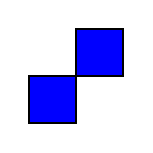
\begin{tikzpicture}
      [%%%%%%%%%%%%%%%%%%%%%%%%%%%%%%
      box/.style={rectangle,draw=black,thick, minimum size=0.6cm},
      ]%%%%%%%%%%%%%%%%%%%%%%%%%%%%%%
      
      \node[box,fill=blue ] at (0.6*0,0.6*0){};  
      \node[box,fill=blue ] at (0.6*1,0.6*1){};  
      % \node[box,fill=blue ] at (0.6*2,0.6*2){};  
      % \node[box,fill=blue ] at (0.6*0,0.6*2){};  
      % \node[box,fill=blue ] at (0.6*2,0.6*0){};  
    \end{tikzpicture}
  \end{minipage}
%  
  \begin{minipage}{2cm}
    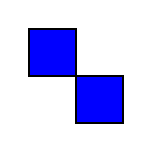
\begin{tikzpicture}
      [%%%%%%%%%%%%%%%%%%%%%%%%%%%%%%
      box/.style={rectangle,draw=black,thick, minimum size=0.6cm},
      ]%%%%%%%%%%%%%%%%%%%%%%%%%%%%%%
      
      % \node[box,fill=blue ] at (0.6*0,0.6*0){};  
      \node[box,fill=blue ] at (0.6*1,0.6*0){};  
      % \node[box,fill=blue ] at (0.6*2,0.6*2){};  
      \node[box,fill=blue ] at (0.6*0,0.6*1){};  
      % \node[box,fill=blue ] at (0.6*2,0.6*0){};  
    \end{tikzpicture}
  \end{minipage}
  %
  \begin{minipage}{3cm}
    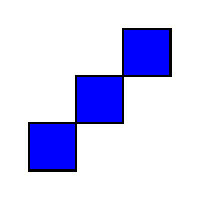
\begin{tikzpicture}
      [%%%%%%%%%%%%%%%%%%%%%%%%%%%%%%
      box/.style={rectangle,draw=black,thick, minimum size=0.6cm},
      ]%%%%%%%%%%%%%%%%%%%%%%%%%%%%%%
      
      \node[box,fill=blue ] at (0.6*0,0.6*0){};  
      \node[box,fill=blue ] at (0.6*1,0.6*1){};  
      \node[box,fill=blue ] at (0.6*2,0.6*2){};  
      % \node[box,fill=blue ] at (0.6*0,0.6*2){};  
      % \node[box,fill=blue ] at (0.6*2,0.6*0){};  
    \end{tikzpicture}
  \end{minipage}
%  
  \begin{minipage}{3cm}
    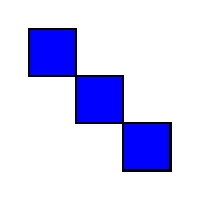
\begin{tikzpicture}
      [%%%%%%%%%%%%%%%%%%%%%%%%%%%%%%
      box/.style={rectangle,draw=black,thick, minimum size=0.6cm},
      ]%%%%%%%%%%%%%%%%%%%%%%%%%%%%%%
      
      % \node[box,fill=blue ] at (0.6*0,0.6*0){};  
      \node[box,fill=blue ] at (0.6*1,0.6*1){};  
      % \node[box,fill=blue ] at (0.6*2,0.6*2){};  
      \node[box,fill=blue ] at (0.6*0,0.6*2){};  
      \node[box,fill=blue ] at (0.6*2,0.6*0){};  
    \end{tikzpicture}
  \end{minipage}

  In the example grids drawn below, the squares with 1 in the input
  array are filled with black color, and all the squares colored blue
  or white are 0 locations. The blue squares visualize a diagonal with
  the biggest possible size that can be fit inside the grid using only
  non-black locations. (Note that there could be multiple possible
  diagonals with the biggest size)

  \begin{minipage}{0.4\textwidth}
    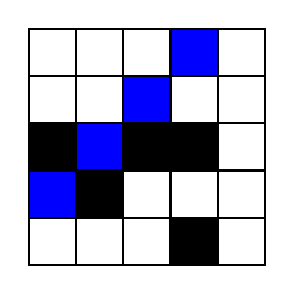
\begin{tikzpicture}
      [%%%%%%%%%%%%%%%%%%%%%%%%%%%%%%
      box/.style={rectangle,draw=black,thick, minimum size=0.6cm},
      ]%%%%%%%%%%%%%%%%%%%%%%%%%%%%%%
      
      \foreach \x in {0,1,...,4}{
        \foreach \y in {0,1,...,4}
        \node[box] at (\x*0.6,\y*0.6){};
      }
      
      \node[box,fill=black ] at (0.6*1,0.6*1){};  
      \node[box,fill=black ] at (0.6*0,0.6*2){};  
      \node[box,fill=black ] at (0.6*3,0.6*0){};  
      \node[box,fill=black ] at (0.6*3,0.6*2){};  
      \node[box,fill=black ] at (0.6*2,0.6*2){};  
      
      \node[box,fill=blue ] at (0.6*0,0.6*1){};  
      \node[box,fill=blue ] at (0.6*1,0.6*2){};  
      % \node[box,fill=blue ] at (0.6*2,0.6*3){};  
      % \node[box,fill=blue ] at (0.6*0,0.6*3){};  
      \node[box,fill=blue ] at (0.6*2,0.6*3){};  
      \node[box,fill=blue ] at (0.6*3,0.6*4){};  
    \end{tikzpicture}
  \end{minipage}
  \begin{minipage}{0.6\textwidth}
    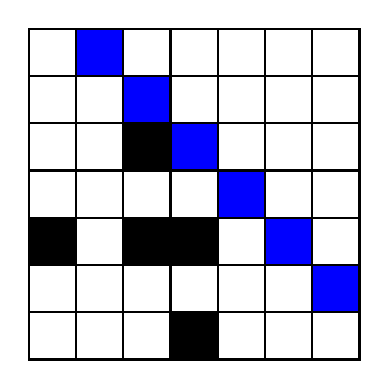
\begin{tikzpicture}
      [%%%%%%%%%%%%%%%%%%%%%%%%%%%%%%
      box/.style={rectangle,draw=black,thick, minimum size=0.6cm},
      ]%%%%%%%%%%%%%%%%%%%%%%%%%%%%%%
      
      \foreach \x in {0,1,...,6}{
        \foreach \y in {0,1,...,6}
        \node[box] at (\x*0.6,\y*0.6){};
      }
      
      \node[box,fill=black ] at (0.6*2,0.6*4){};  
      \node[box,fill=black ] at (0.6*0,0.6*2){};  
      \node[box,fill=black ] at (0.6*3,0.6*0){};  
      \node[box,fill=black ] at (0.6*3,0.6*2){};  
      \node[box,fill=black ] at (0.6*2,0.6*2){};  
      
      % \node[box,fill=blue ] at (0.6*2,0.6*1){};  
      % \node[box,fill=blue ] at (0.6*3,0.6*2){};  
      \node[box,fill=blue ] at (0.6*1,0.6*6){};  
      \node[box,fill=blue ] at (0.6*4,0.6*3){};  
      % \node[box,fill=blue ] at (0.6*5,0.6*4){};  
      % \node[box,fill=blue ] at (0.6*6,0.6*5){};  
      \node[box,fill=blue ] at (0.6*2,0.6*5){};  
      \node[box,fill=blue ] at (0.6*3,0.6*4){};  
      \node[box,fill=blue ] at (0.6*5,0.6*2){};  
      \node[box,fill=blue ] at (0.6*6,0.6*1){};  
    \end{tikzpicture}
  \end{minipage}
  Thus the expected answers for the above two examples are 4 and 6.
  
  
  Design an algorithm for the above problem with a worst case
  running-time complexity of $O(n^2)$ following the steps below.
  \begin{enumerate}
  \item \textbf{[1 point]} Clearly and precisely specify in English
    the problem you wish to solve.
  \item \textbf{[4 points]} Give a recursive solution for the
    problem (including base cases) and justify it. (Hint: You may
    need to define more than one recursive function)
  \item \textbf{[1 point]} Specify all the subproblems that your
    algorithm needs to solve.
  \item \textbf{[3 point]} Specify the memoization data structure(s),
    clearly define what value will be stored in each location at the
    end of the algorithm, and give a good bottom-up evaluation order
    for filling the memoization datastructure(s).
  \item \textbf{[6 point]} Write down the final
    dynamic-programming algorithm (non-recursive), and analyze its
    time and space complexity.
  \end{enumerate}
  \medskip
  \medskip

      
\item \textbf{[15 points]}

  The pandemic unleashed due to the SARS-CoV-2 virus (also referred to
  as Covid-19) has resulted in mandatory social distancing
  requirements.

  As the University plans to reopen its classrooms to be used for
  in-person lectures again, it needs to ensure that the physical
  distancing guidelines are followed. 
  %
  As a result, the university needs to reconsider the layout of its
  classrooms.
  %

  Assume that each student seat is exactly 1 feet wide.
  %
  As per the distancing requirement, every two seated students must
  have at least 6 feet of distance between them.
  %
  You are intrigued, and want to count the resulting number of
  possible student seating arrangements.

  For some $n \ge 0,$ consider a row with exactly $n+1$ seats.
  %
  You are given an array of $n$ non-negative integers
  $\texttt{A[1...n]}$, where $\texttt{A[i]}$ gives the distance in feet
  between seat $i$ and seat $i+1.$
  %

  Your goal is to determine the number of possible valid student
  seating arrangements.

  e.g. Given \texttt{A = [2, 3]}, specifying the distances between 3
  seats, there are a total of 5 valid seating arrangements:
  \begin{itemize}
  \item 1 arrangement with no students
    \texttt{\textvisiblespace\textvisiblespace\textvisiblespace}, 
  \item 3 possible arrangements with 1 student
    \texttt{X\textvisiblespace\textvisiblespace},
    \texttt{\textvisiblespace X\textvisiblespace},
    \texttt{\textvisiblespace\textvisiblespace X}, 
  \item and one arrangement with 2 students \texttt{X\textvisiblespace
      X}.
  \end{itemize}
  Note that the last arrangement is valid since the empty seat in the
  middle is 1 feet wide, giving that the distance between the two
  students is exactly 6 feet.

  Systematically design a Dynamic Programming based algorithm for the
  above problem with worst case running-time complexity of $O(n)$ by
  answering the following questions:
  \begin{enumerate}
  \item \textbf{[1 point]} Clearly and precisely specify in English the
    problem you wish to solve recursively.
  \item \textbf{[3 point]} Give a clear and precise recursive formula
    / algorithm for solving the problem and justification for its
    correctness. Identify and specify the base cases.
  \item \textbf{[1 point]} Identify all the subproblems that your
    recursive algorithm needs to solve.
  \item \textbf{[1 point]} What is the memoization data structure you will use?
  \item \textbf{[2 point]} Find a good bottom-up evaluation order of the
    memoization data-structure (non-recursive) such that before
    solving a subproblem instance, all necessary subproblems have been
    solved.
  \item \textbf{[5 point]} Write down the final dynamic-programming
    algorithm (non-recursive).
  \item \textbf{[2 point]} Analyze its time and space complexity.
  \end{enumerate}
  

\item \textbf{[15 points]}
      
  You are given an array $S$ of $n$ distinct numbers (not necessarily
  integers) in sorted order such that all numbers in $S$ are
  non-negative, i.e.  $a \ge 0$ for all $a \in S.$ You are also given
  a target value $V.$ Your goal is to determine the number of distinct
  pairs $(a, b)$ such that $a, b \in S$ and $a \neq b$ such that
  \begin{equation*}
    a^4 + b^4 + 4ab \le V.
  \end{equation*}
We will consider $(a, b)$ to be the same pair
as $(b, a).$ e.g.
Given $S = [4, 6, 7, 9, 11],$ and $V = 3865,$ the answer is 3
(consider the pairs $(4,6),(4,7),(6, 7)$), and if $V = 1000,$ the answer is 0.

Systematically design an algorithm for this problem that has a
worst-case time complexity of $O(n).$  Note: you're not allowed to use
a formula for solving the quartic equation.
\begin{enumerate}
\item \textbf{(3 points)} Clearly describe all the subproblems that
  will be solved by your algorithm, and the values that will be stored
  in all the data-structure being used by your algorithm.
\item \textbf{(5 points)} Write your algorithm in pseudo-code and
  analyze its complexity.
\item \textbf{(7 points)} Give a convincing proof of correctness for
  your algorithm. Remember that if your algorithm is greedy, you will
  not get any marks for the previous parts without a proof of correctness.
\end{enumerate}

\end{enumerate}

\end{document}

%%% Local Variables:
%%% mode: latex
%%% TeX-master: t
%%% End:
